\documentclass[10pt]{article}
\usepackage[paperwidth=11.8cm,paperheight=4.5cm,margin=0pt]{geometry}
\usepackage{tikz}
\usepackage{amsmath,amssymb}
\usepackage{mathptmx}
\pagestyle{empty}
\begin{document}
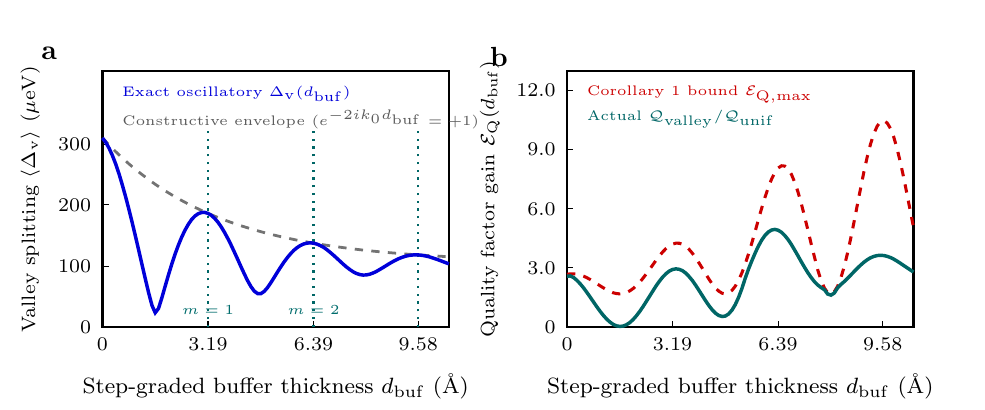
\begin{tikzpicture}[x=1cm,y=1cm]
  \useasboundingbox (0,0) rectangle (11.8,4.5);

  % Panel a: Mean Valley Splitting vs Buffer Thickness d_buf
  \node[anchor=north west,font=\bfseries\normalsize] at (0.05,4.38) {a};
  \draw[thick] (0.95,0.70) rectangle (5.35,3.95);
  \foreach \v/\y in {0/0.70, 100/1.47, 200/2.25, 300/3.02} {
    \draw (0.95,\y) -- (1.03,\y);
    \node[left,font=\scriptsize] at (0.93,\y) {\v};
  }
  \foreach \xval/\xpos in {0/0.95, 3.19/2.29, 6.39/3.63, 9.58/4.96} {
    \draw (\xpos,0.70) -- (\xpos,0.78);
    \node[below,font=\scriptsize] at (\xpos,0.68) {\xval};
  }
  \node[below,font=\footnotesize] at (3.15,0.22) {Step-graded buffer thickness $d_{\mathrm{buf}}$ ($\text{\AA}$)};
  \node[rotate=90,above,font=\scriptsize] at (0.28,2.32) {Valley splitting $\langle\Delta_{\mathrm{v}}\rangle$ ($\mu\mathrm{eV}$)};

  % Vertical resonant lines m=1,2,3
  \draw[dotted,teal!80!black,thick] (2.29,0.70) -- (2.29,3.20);
  \draw[dotted,teal!80!black,thick] (3.63,0.70) -- (3.63,3.20);
  \draw[dotted,teal!80!black,thick] (4.96,0.70) -- (4.96,3.20);

  \draw[black!55,dashed,line width=1.0pt] (0.950,3.099) -- (1.034,3.010) -- (1.118,2.925) -- (1.201,2.846) -- (1.285,2.771) -- (1.369,2.700) -- (1.453,2.634) -- (1.537,2.571) -- (1.620,2.511) -- (1.704,2.455) -- (1.788,2.402) -- (1.872,2.352) -- (1.956,2.305) -- (2.040,2.260) -- (2.123,2.219) -- (2.207,2.179) -- (2.291,2.142) -- (2.375,2.106) -- (2.459,2.073) -- (2.542,2.042) -- (2.626,2.012) -- (2.710,1.984) -- (2.794,1.958) -- (2.878,1.933) -- (2.961,1.909) -- (3.045,1.887) -- (3.129,1.866) -- (3.213,1.846) -- (3.297,1.828) -- (3.380,1.810) -- (3.464,1.793) -- (3.548,1.778) -- (3.632,1.763) -- (3.716,1.749) -- (3.800,1.736) -- (3.883,1.724) -- (3.967,1.712) -- (4.051,1.701) -- (4.135,1.690) -- (4.219,1.680) -- (4.302,1.671) -- (4.386,1.662) -- (4.470,1.654) -- (4.554,1.646) -- (4.638,1.639) -- (4.721,1.632) -- (4.805,1.625) -- (4.889,1.619) -- (4.973,1.613) -- (5.057,1.608) -- (5.140,1.603) -- (5.224,1.598) -- (5.308,1.593);
  \draw[blue!85!black,line width=1.25pt] (0.950,3.099) -- (0.992,3.043) -- (1.034,2.969) -- (1.076,2.877) -- (1.118,2.768) -- (1.160,2.644) -- (1.201,2.506) -- (1.243,2.356) -- (1.285,2.195) -- (1.327,2.026) -- (1.369,1.850) -- (1.411,1.670) -- (1.453,1.487) -- (1.495,1.306) -- (1.537,1.130) -- (1.579,0.972) -- (1.620,0.880) -- (1.662,0.935) -- (1.704,1.069) -- (1.746,1.216) -- (1.788,1.360) -- (1.830,1.497) -- (1.872,1.624) -- (1.914,1.738) -- (1.956,1.840) -- (1.998,1.928) -- (2.040,2.002) -- (2.081,2.062) -- (2.123,2.107) -- (2.165,2.137) -- (2.207,2.152) -- (2.249,2.154) -- (2.291,2.141) -- (2.333,2.116) -- (2.375,2.078) -- (2.417,2.029) -- (2.459,1.969) -- (2.500,1.900) -- (2.542,1.822) -- (2.584,1.738) -- (2.626,1.648) -- (2.668,1.556) -- (2.710,1.462) -- (2.752,1.371) -- (2.794,1.285) -- (2.836,1.211) -- (2.878,1.154) -- (2.920,1.123) -- (2.961,1.122) -- (3.003,1.150) -- (3.045,1.198) -- (3.087,1.259) -- (3.129,1.326) -- (3.171,1.394) -- (3.213,1.460) -- (3.255,1.523) -- (3.297,1.579) -- (3.339,1.629) -- (3.380,1.672) -- (3.422,1.707) -- (3.464,1.734) -- (3.506,1.753) -- (3.548,1.764) -- (3.590,1.767) -- (3.632,1.763) -- (3.674,1.751) -- (3.716,1.733) -- (3.758,1.710) -- (3.800,1.681) -- (3.841,1.647) -- (3.883,1.611) -- (3.925,1.573) -- (3.967,1.534) -- (4.009,1.495) -- (4.051,1.459) -- (4.093,1.427) -- (4.135,1.399) -- (4.177,1.378) -- (4.219,1.364) -- (4.260,1.358) -- (4.302,1.360) -- (4.344,1.369) -- (4.386,1.384) -- (4.428,1.404) -- (4.470,1.428) -- (4.512,1.453) -- (4.554,1.479) -- (4.596,1.505) -- (4.638,1.529) -- (4.680,1.551) -- (4.721,1.570) -- (4.763,1.586) -- (4.805,1.599) -- (4.847,1.608) -- (4.889,1.613) -- (4.931,1.615) -- (4.973,1.613) -- (5.015,1.608) -- (5.057,1.600) -- (5.099,1.590) -- (5.140,1.577) -- (5.182,1.563) -- (5.224,1.548) -- (5.266,1.532) -- (5.308,1.516) -- (5.350,1.501);

  \node[anchor=north west,font=\tiny,blue!85!black] at (1.08,3.88) {Exact oscillatory $\Delta_{\mathrm{v}}(d_{\mathrm{buf}})$};
  \node[anchor=north west,font=\tiny,black!65] at (1.08,3.58) {Constructive envelope ($e^{-2ik_0d_{\mathrm{buf}}}=+1$)};
  \node[font=\tiny,teal!85!black] at (2.29,0.92) {$m=1$};
  \node[font=\tiny,teal!85!black] at (3.63,0.92) {$m=2$};

  % Panel b: Valley Coherence Quality Factor Enhancement E_Q(d_buf)
  \node[anchor=north west,font=\bfseries\normalsize] at (5.75,4.38) {b};
  \draw[thick] (6.85,0.70) rectangle (11.25,3.95);
  \foreach \v/\y in {0/0.70, 3.0/1.45, 6.0/2.20, 9.0/2.95, 12.0/3.70} {
    \draw (6.85,\y) -- (6.93,\y);
    \node[left,font=\scriptsize] at (6.83,\y) {\v};
  }
  \foreach \xval/\xpos in {0/6.85, 3.19/8.19, 6.39/9.53, 9.58/10.86} {
    \draw (\xpos,0.70) -- (\xpos,0.78);
    \node[below,font=\scriptsize] at (\xpos,0.68) {\xval};
  }
  \node[below,font=\footnotesize] at (9.05,0.22) {Step-graded buffer thickness $d_{\mathrm{buf}}$ ($\text{\AA}$)};
  \node[rotate=90,above,font=\scriptsize] at (6.12,2.32) {Quality factor gain $\mathcal{E}_{\mathrm{Q}}(d_{\mathrm{buf}})$};

  \draw[red!80!black,dashed,line width=1.1pt] (6.850,1.369) -- (6.892,1.374) -- (6.934,1.374) -- (6.976,1.369) -- (7.018,1.359) -- (7.060,1.344) -- (7.101,1.325) -- (7.143,1.302) -- (7.185,1.277) -- (7.227,1.250) -- (7.269,1.222) -- (7.311,1.196) -- (7.353,1.171) -- (7.395,1.150) -- (7.437,1.133) -- (7.479,1.123) -- (7.520,1.119) -- (7.562,1.124) -- (7.604,1.136) -- (7.646,1.157) -- (7.688,1.186) -- (7.730,1.223) -- (7.772,1.267) -- (7.814,1.317) -- (7.856,1.373) -- (7.898,1.430) -- (7.940,1.489) -- (7.981,1.547) -- (8.023,1.602) -- (8.065,1.652) -- (8.107,1.695) -- (8.149,1.728) -- (8.191,1.752) -- (8.233,1.763) -- (8.275,1.762) -- (8.317,1.749) -- (8.359,1.722) -- (8.400,1.684) -- (8.442,1.635) -- (8.484,1.577) -- (8.526,1.512) -- (8.568,1.444) -- (8.610,1.374) -- (8.652,1.307) -- (8.694,1.245) -- (8.736,1.193) -- (8.778,1.153) -- (8.820,1.127) -- (8.861,1.119) -- (8.903,1.131) -- (8.945,1.164) -- (8.987,1.218) -- (9.029,1.293) -- (9.071,1.387) -- (9.113,1.500) -- (9.155,1.628) -- (9.197,1.767) -- (9.239,1.913) -- (9.280,2.062) -- (9.322,2.208) -- (9.364,2.346) -- (9.406,2.471) -- (9.448,2.578) -- (9.490,2.662) -- (9.532,2.719) -- (9.574,2.746) -- (9.616,2.742) -- (9.658,2.705) -- (9.700,2.636) -- (9.741,2.538) -- (9.783,2.413) -- (9.825,2.265) -- (9.867,2.101) -- (9.909,1.928) -- (9.951,1.752) -- (9.993,1.583) -- (10.035,1.420) -- (10.077,1.288) -- (10.119,1.192) -- (10.160,1.135) -- (10.202,1.120) -- (10.244,1.147) -- (10.286,1.216) -- (10.328,1.324) -- (10.370,1.466) -- (10.412,1.637) -- (10.454,1.831) -- (10.496,2.040) -- (10.538,2.256) -- (10.580,2.470) -- (10.621,2.674) -- (10.663,2.862) -- (10.705,3.024) -- (10.747,3.155) -- (10.789,3.250) -- (10.831,3.306) -- (10.873,3.319) -- (10.915,3.290) -- (10.957,3.221) -- (10.999,3.112) -- (11.040,2.968) -- (11.082,2.796) -- (11.124,2.602) -- (11.166,2.393) -- (11.208,2.178) -- (11.250,1.964);
  \draw[teal!80!black,line width=1.25pt] (6.850,1.343) -- (6.892,1.347) -- (6.934,1.326) -- (6.976,1.290) -- (7.018,1.246) -- (7.060,1.195) -- (7.101,1.139) -- (7.143,1.079) -- (7.185,1.018) -- (7.227,0.957) -- (7.269,0.899) -- (7.311,0.846) -- (7.353,0.799) -- (7.395,0.761) -- (7.437,0.731) -- (7.479,0.713) -- (7.520,0.706) -- (7.562,0.710) -- (7.604,0.727) -- (7.646,0.754) -- (7.688,0.792) -- (7.730,0.840) -- (7.772,0.895) -- (7.814,0.956) -- (7.856,1.022) -- (7.898,1.089) -- (7.940,1.156) -- (7.981,1.221) -- (8.023,1.280) -- (8.065,1.333) -- (8.107,1.376) -- (8.149,1.409) -- (8.191,1.429) -- (8.233,1.437) -- (8.275,1.431) -- (8.317,1.413) -- (8.359,1.382) -- (8.400,1.339) -- (8.442,1.288) -- (8.484,1.228) -- (8.526,1.163) -- (8.568,1.097) -- (8.610,1.031) -- (8.652,0.970) -- (8.694,0.916) -- (8.736,0.873) -- (8.778,0.844) -- (8.820,0.832) -- (8.861,0.838) -- (8.903,0.865) -- (8.945,0.914) -- (8.987,0.984) -- (9.029,1.076) -- (9.071,1.188) -- (9.113,1.318) -- (9.155,1.435) -- (9.197,1.540) -- (9.239,1.638) -- (9.280,1.726) -- (9.322,1.802) -- (9.364,1.862) -- (9.406,1.905) -- (9.448,1.930) -- (9.490,1.938) -- (9.532,1.927) -- (9.574,1.901) -- (9.616,1.860) -- (9.658,1.807) -- (9.700,1.744) -- (9.741,1.675) -- (9.783,1.602) -- (9.825,1.527) -- (9.867,1.455) -- (9.909,1.387) -- (9.951,1.326) -- (9.993,1.273) -- (10.035,1.231) -- (10.077,1.199) -- (10.119,1.172) -- (10.160,1.117) -- (10.202,1.103) -- (10.244,1.130) -- (10.286,1.196) -- (10.328,1.239) -- (10.370,1.275) -- (10.412,1.316) -- (10.454,1.359) -- (10.496,1.403) -- (10.538,1.446) -- (10.580,1.486) -- (10.621,1.522) -- (10.663,1.553) -- (10.705,1.578) -- (10.747,1.595) -- (10.789,1.606) -- (10.831,1.609) -- (10.873,1.606) -- (10.915,1.596) -- (10.957,1.581) -- (10.999,1.560) -- (11.040,1.536) -- (11.082,1.509) -- (11.124,1.480) -- (11.166,1.452) -- (11.208,1.424) -- (11.250,1.397);

  \node[anchor=north west,font=\tiny,red!80!black] at (6.98,3.88) {Corollary 1 bound $\mathcal{E}_{\mathrm{Q},\max}$};
  \node[anchor=north west,font=\tiny,teal!80!black] at (6.98,3.58) {Actual $\mathcal{Q}_{\mathrm{valley}}/\mathcal{Q}_{\mathrm{unif}}$};
\end{tikzpicture}
\end{document}
